\section{Исследование и построение решения задачи}
\label{sec:Section3} \index{Section3}

% \subsection{Устройство архитектуры процессор-память}

% \subsubsection{Микроархитектура процессора}

%     Современный ЦП (центральный процессор) представляет собой
%     систему взаимосвязанных между собой процессорных ядер, не обязательно одинаковых.

%     Исполнение инструкции современным процессорным ядром является многостадийным конвейером
%     из различных блоков. В зависимости от исполняемой рабочей нагрузки утилизируются различные блоки
%     процессора, поэтому скорость исполнения таковой рабочей нагрузки сильно зависит
%     от её особенностей (типа) и особенностей исполнения таковых нагрузок на блоках процессора.

%     В наиболее общем виде можно разбить конвейер исполнения инструкции на процессоре на несколько
%     последовательных стадий:
%     \begin{enumerate}
%         \item Чтение инструкции из памяти;
%         \item Декодирование прочитанной инструкции;
%         \item Исполнение инструкции на вычислительных блоках;
%         \item Чтение/запись в память при необходимости;
%         \item Запись результата исполнения инструкции в регистры процессора.
%     \end{enumerate}

%     Чаще всего приведённые выше стадии дробятся на более локальные стадии, применяются
%     дополнительные оптимизации для ускорения исполнения инструкций а также их распараллеливания
%     (например, кеширование декодированных инструкций и предсказатель ветвлений). Наиболее
%     актуальным примером являются OoO (Out-of-Order -- внеочередное или спекулятивное исполнение)
%     процессоры, в которых используется алгоритм Томасуло, позволяющий реализовать
%     исполнение машинных инструкций не в порядке их следования в машинном коде, а в порядке
%     готовности к выполнению, за счёт чего значительно увеличивается скорость исполнения инструкций.

%     В типичной реализации OoO используется ROB (Re-order buffer), который представляет собой
%     циклический буфер и накапливает инструкции для обеспечения возможности их переупорядочить.
%     Обычно в ROB попадают не исходные машинные иструкции, а прошедшие через стадию переименование
%     регистров для избавления от зависимостей по данным (для дополнительного распараллеливания
%     инструкций).

%     Наибольший интерес в данной работе представляет организация обращения процессора в память,
%     также затрагиваются аспекты, связанные с OoO исполнением.

%     \begin{figure}[!h]
%         \caption{Схема конвейера процессора Arm Cortex A77 \cite{CortexA77Docs}}
%         \centering
%         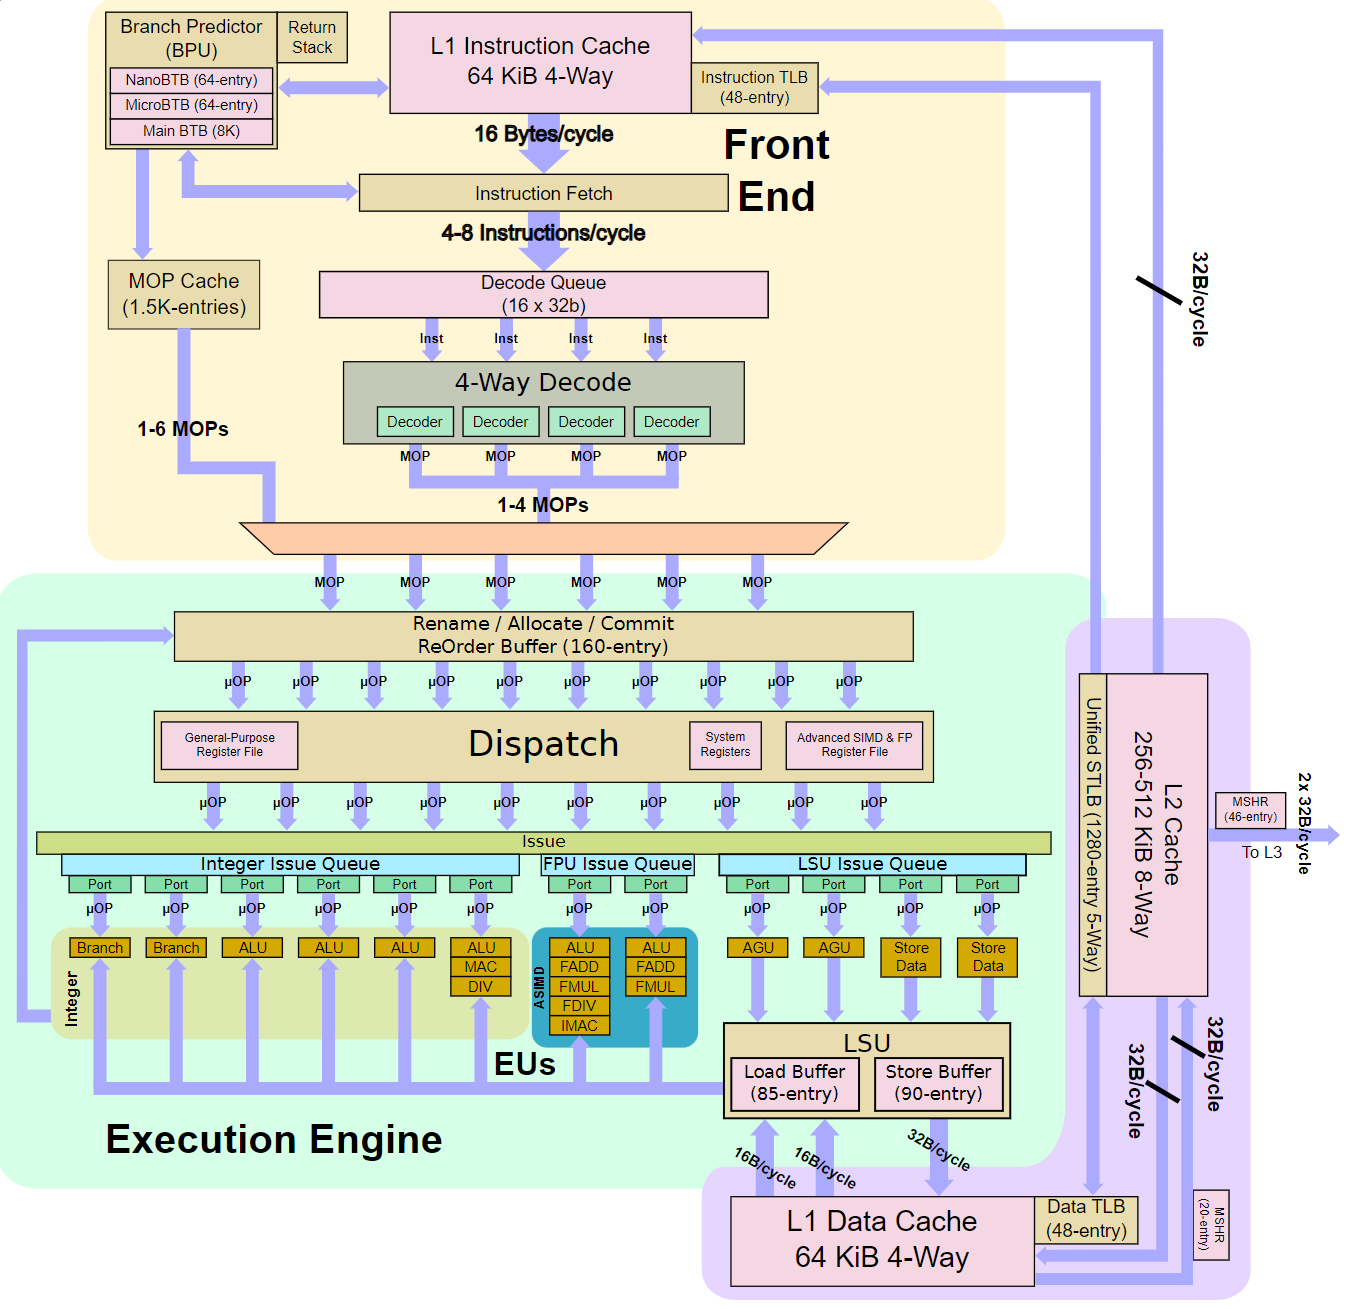
\includegraphics[width=161mm]{CortexA77}
%         \label{cortexA77}
%     \end{figure}

% \subsubsection{Организация системы памяти}

%     Процессор в современных мобильных системах встроен в так называемую SoC (System-on-chip --
%     система на кристалле) систему -- электронная схема, которая выполняет цели компьютера
%     и размещена на одной интегральной схеме. Таким образом, в такую систему встроены сразу процессор,
%     таймеры, счётчики, интерфейсы для периферийных устройств, ОЗУ, ПЗУ и даже графический ускоритель.
%     Именно таким образом устроены современные
%     смартфоны, фотоаппараты, умные часы, элекронные книги и схожие устройства.

%     Одна из основных подсистем системы на кристалле -- подсистема памяти. Наиболее быстродействующими
%     элементами памяти являются регистры процессора, они же имеют наименьшее количество памяти, более
%     высокую цену для производства и самую малую плотность расположения в электронной схеме.

%     Учитывая малый объём возможного хранения данных с помощью регистров, а также
%     что любая вычислительная система обладает локальностью (как по данным, так и по
%     времени), почти всегда вводят дополнительные уровни памяти -- более дешёвые в производстве,
%     имеющий больший объём и более высокую плотность ячеек хранения данных на электронной схеме.
%     Более низкие уровни памяти являются кешами для более высоких.
%     Таким образом, любая система имеет ОЗУ и кеши в качестве промежуточного хранилища данных
%     (см. рис. \ref{CachePyramid}).

%     Во всех современных мобильных системах в качестве ОЗУ используется LPDDR SDRAM
%     (Low-Power Double Data Rate Synchronous Dynamic Random-Access Memory --
%     динамическая оперативная память синхронного доступа с двойной скоростью передачи данных и
%     с низким энергопотреблением). В дальнейшем для удобства будем использовать более простое
%     обозначение для такой памяти -- DDR (Double Data Rate) память.

%     Количество уровней кешей и объём их памяти напрямую зависят от требований к исполнению
%     современных приложений и особенностей архитектуры мобильной системы,
%     всегда являются компромиссом: с одной стороны, добавление дополнительного
%     уровня кеша -- снижение вероятности обращения в DDR память (наиболее медленная память),
%     а с другой -- введение постоянной дополнительной задержки при обращении в DDR, если данные
%     в кешах отсутствуют.

%     \begin{figure}[!h]
%         \caption{Пример иерархии памяти в системе с 3-мя уровнями кешей}
%         \centering
%         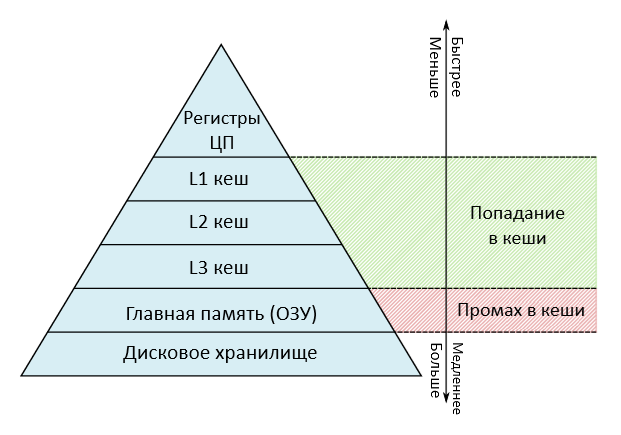
\includegraphics[width=116mm]{CachePyramidRU}
%         \label{CachePyramid}
%     \end{figure}

%     Чаще всего производят мобильные устройства с 2-мя и более уровнями кешей. В системах на кристалле,
%     как правило, последним (дополнительным) уровнем является системный кеш, который обычно
%     не вносят в список уровней кешей процессора, так как он используется не только самим процессором,
%     но также и различными периферийными устройствами, такими как графический ускоритель, ускоритель
%     нейронных сетей и т.д..

%     \begin{figure}[!h]
%         \caption{Пример иерархии кешей в многоядерном процессоре (отсутствуют кеш 3-его уровня
%             и системный кеш)}
%         \centering
%         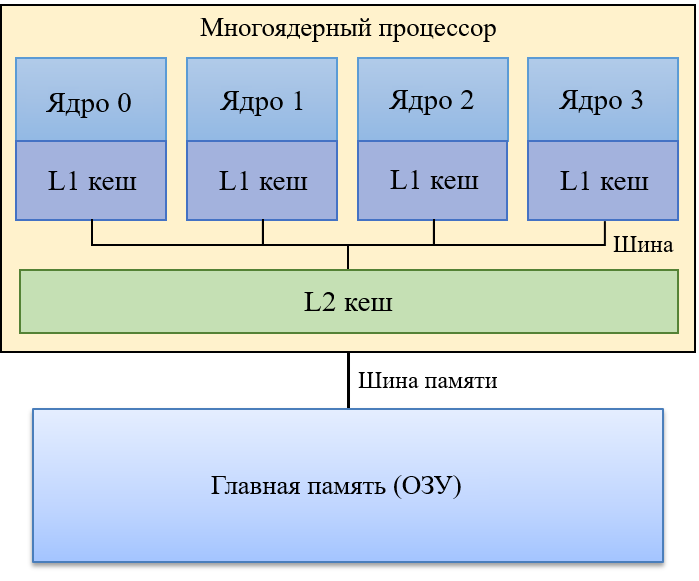
\includegraphics[width=95mm]{MulticoreCacheRU}
%         \label{MulticoreCache}
%     \end{figure}

%     Каждое ядро процессора имеет кеш инструкций и кеш данных 1-ых уровней, на которые для краткости
%     ссылаются как на единый кеш 1-ого уровня.
%     При промахе в кеш 1-ого уровня поиск данных происходит в кеше 2-ого уровня, при промахе
%     в кеш 2-ого -- поиск в кеше 3-его (если таковой имеется), и так до тех пор, пока не возникнет
%     промах в системный кеш, после чего произойдёт обращение в DDR память
%     (см. рис. \ref{MulticoreCache}).

%     Как правило, кеш 2-ого уровня уникален для каждого ядра, хотя в некоторых гетерогенных системах
%     кеш 2-ого уровня может использовать либо группой из 2-ух ядер в марках 1-ого кластера, либо
%     целиком всем кластером ядер (такое поведение характерно для энергоэффективных ядер).
%     Кеш 3-его уровня всегда разделяется между всеми ядрами системы, как и системный кеш вместе с ОЗУ.

%     ПЗУ, а также компоненты для долгосрочного хранения данных (диски, твёрдотельные накопители и др.)
%     в данной работе рассматриваться не будут.

% \subsubsection{Латентность памяти и утилизация её пропускной способности} \label{lat_util_chapter}

%     Для построения модели производительности ядра процессора, т.е. для правильного подсчёта утилизации
%     ядра и наиболее энергоэффективного регулирования частотами, важно учитывать не только структуру
%     организации памяти в исследуемой системе, а также и динамические характеристики элементов
%     такой системы. Наиболее важными характеристиками являются пропускная способность шин,
%     соединяющих вычислительные подсистемы с подсистемами памяти, утилизация пропускной способности и
%     латетность памяти -- промежуток времени между отправлением запроса на получение данных в память и
%     между самим получением данных.

%     Таким образом, кеши и DDR память имеют свои собственные динамические характеристики,
%     приведённые ранее. Как правило, низкие уровни кешей работают на той же частоте, что
%     и само процессорное ядро (группа ядер -- ядерный кластер), поэтому латентность таких кешей
%     выражается через циклы ядра процессора, а не через абсолютное время. Сложнее ситуация обстоит
%     с более высокими уровнями кешей и DDR памятью: они имеют отдельные источники тактирования,
%     латентность выражается в аболютном времени, к тому же она зависит от утилизации
%     пропускной способности шин, ведущих к этим элементам памяти, то есть от количества транзакций
%     в единицу времени.

%     В данной работе часть предлагаемой модели требует использования латентности памяти, поэтому
%     необходимо рассмотреть существующие решения для её определения и/или возможного учёта в модели.

%     Авторы работы \cite{keramidas2010interval} предлагают 2 модели для учёта латентности памяти
%     в рамках алгоритма регулирования частот. Первая модель разбивает циклы процессора на 2
%     компоненты: относящиеся к ожиданию транзакций памяти и
%     относящиеся непосредственно к вычислительным блокам ядра процессора.
%     Утверждается, что при изменении частоты ядра процессора изменяются только циклы, относящиеся к памяти
%     (частота которой независима от частоты ядра).
%     На этом и основывается алгоритм регулирования частот, использующий перерасчёт времени
%     исполнения через циклы при различных частотах. Вторая модель является модификацией-улучшением
%     первой модели: дополнительно предполагается, что в группе инструкций, которые обращаются в
%     память подряд, следует учитывать только первую инструкцию в формуле для перерасчёта циклов,
%     которые относятся к памяти, однако это требует наличие дополнительной информации на уровне кешей:
%     среди всех промахов в кеши (т.е. обращений в следующий уровень памяти) следует учитывать только
%     первые промахи среди группы промахов (промахов, находящихся на расстоянии порядка времени
%     латентности обращения в вышележащие уровни памяти), что не поддерживается ни одним устройством.

%     В работе также отмечается, что следует учитывать ROB в OoO процессорах: из циклов, относящихся к
%     транзакциям памяти, следует вычесть ту часть циклов, которую тратит процессор на исполнение
%     инструкций, расположенных в логическом порядке после инструкции-обращения в память,
%     так как такие инструкции исполняются спекулятивно.

%     В работе \cite{clapp2015quantifying} рассматривается подход использования аналитической
%     формулы влияния утилизации пропускной способности памяти на её латентность, что влияет
%     на производительность суперскалярного процессора в рамках рабочих нагрузок,
%     связанных с областью вычислений больших данных.
%     В этом подходе используется схожий принцип, предлагаемых в данной работе: использование как
%     показателя производительности $cpi$ (отношения числа процессорных циклов к числу исполненных
%     инструкций), которое включает в себя слагаемые, связанные с циклами, потраченными
%     на время ожидания транзакций-обращений в память. Авторы вводят понятие блокирующего фактора
%     для латентности: в зависимости от рабочей нагрузки при одинаковом количестве обращений в память
%     влияние латентности на производительность ($cpi$) может меняться вплоть до десятка раз из-за
%     параллельных обращений в память, что коррелирует с результатами работы \cite{keramidas2010interval}.
%     При фиксированном блокирующем факторе значение $cpi$ зависит линейно от количества обращений
%     в память в единицу инструкций.
%     Таким образом, все рабочие нагрузки разделены на 2 вида: чувствительные к латентности (высокое
%     значение блокирующего фактора) и чуствительные к пропускной способности (низкое значение
%     блокирующего фактора).
%     Однако данное исследование ограничивается
%     рассмотрением обращений только в DDR память при фиксированных частотах всех устройств.

%     Авторы работы \cite{eyerman2022dram} предлагает метод визуализации утилизации пропускной способности
%     ОЗУ для выявления возможных мест оптимизации производительности: для этого они используют
%     контроллер внутри ОЗУ для вычисления утилизации пропускной способности и латентности.

%     Зависимость латентности от утилизации пропускной способности представляет собой монотонную
%     возрастающую функцию, которую можно положить константой при значениях утилизации, не сильно близкой
%     к максимально возможной (\cite{david2011memory}), при приближении утилизации к своему максимуму
%     латентность начинает сильно расти.

%     Таким образом, можно сделать основные выводы из существующих работ:
%     \begin{enumerate}
%         \item Чувствительность производительности к латентности памяти зависит от рабочей нагрузки и может
%             быть очень низкой даже при большом количестве обращений в память (ОЗУ). Такая зависимость
%             определяется уровнем параллелизма обращений в память.
%         \item Латентность является монотонной возрастающей функцией от утилизации пропускной способности,
%             которую можно приближённо положить константой почти на всём интеравале утилизации;
%             при стремлении утилизации к своему пределу происходит быстрый рост латентности до значений,
%             на порядки превышающих её нормальное значение.
%     \end{enumerate}

\subsection{Описание модели производительности процессора}

    Главной характеристикой производительности процессора является количество инструкций,
    исполняемых в еденицу времени -- чем больше это значение, тем быстрее исполняется рабочая
    нагрузка (приложение). Причём заданное количество инструкций исполняется за разное количество
    процессорных циклов, которые, в свою очередь, обратно пропорциональны времени исполнения
    этих инструкций.

    Пусть за время $\tau$ процессор непрерывно исполнял инструкции и исполнил $instrs$ инструкций
    за $cycles$ циклов при заданной частоте процессора $freq_{cpu}$.
    Тогда, очевидно, выполняется следующее соотношение:

    \begin{equation} \label{cycles_base}
        cycles = \frac{freq_{cpu}}{\tau}
    \end{equation}

    На практике чаще всего используют такие величины как $cpi = cycles / instrs$ и
    $ipc = instrs / cycles$ в качестве меры производительности процессора: чем выше/ниже значение
    $ipc$/$cpi$, тем лучше процессор. Однако кроме типа процессорного ядра на эти значения также
    влияют частота самого ядра и частоты остальных компонент системы. Например, при повышении частоты
    процессора величина $ipc$ либо остаётся такой же, если отсутствуют инструкции, связанные с
    обращением высокие уровни памяти (ОЗУ или кеши высокого уровня), либо уменьшается, если
    процессор часто обращается в кеши высокого уровня или оперативную память, из-за чего циклы тратятся
    впустую.

    За время $\tau$ процессор часть циклов тратит на исполнение инструкций непосредственно на
    процессорных блоках (в том числе вычислительных), а оставшуюся часть на ожидание операций,
    связанных с обращением в память (в кеши или оперативную память): обозначим эти величины
    $cycles_{cpu}$ и $cycles_{mem}$, тогда справедливо

    \begin{equation}
        cpi = \frac{cycles}{instrs} = \frac{cycles_{cpu}}{instrs} + \frac{cycles_{mem}}{instrs}
    \end{equation}

    Важно отметить, что $\frac{cycles_{cpu}}{instrs}$ -- значение $cpi$, если бы все обращения
    в кеши и оперативную память занимали 0 циклов, т.е. эти работали бы бесконечно быстро, а значит
    количество циклов ограничивалось снизу возможностями процессора. Обозначим данное соотношение
    как $cpi_{cpu} \equiv \frac{cycles_{cpu}}{instrs}$.

    В свою очередь величина $cycles_{mem}$ характеризуется только лишь внешними компонентами системы,
    не зависящими от конвейера ядра процессора. Пусть, например, если имеется 2 уровня кешей и оперативная память.
    Время доступа к определённому уровню кеша характеризуется средней величиной $cycles_{L_{i}}$,
    представляющую собой латентность кеша (время задержки обращения), выраженную в процессорных
    циклах, где $i$ -- номер уровня кеша.
    После обращения в кеш возможны 2 ситуации: либо попадание к кеш, либо промах и обращение в
    следующий уровень кеша или оперативную память.
    Время доступа к оперативной памяти обозначим $cycles_{ram}$.

    Выражая времена доступа через собственные частоты и латентности, получим:

    \begin{equation}
        cycles_{mem} = n_{L_1} \cdot \frac{lat_{L_1}}{freq_{L_1}} \cdot freq_{cpu} +
        n_{L_2} \cdot \frac{lat_{L_2}}{freq_{L_2}} \cdot freq_{cpu} +
        n_{ram} \cdot \frac{lat_{ram}}{freq_{ram}} \cdot freq_{cpu},
    \end{equation}

    \begin{equation}
        cpi = cpi_{cpu} + \frac{n_{L_1} \cdot \frac{lat_{L_1}}{freq_{L_1}} +
        n_{L_2} \cdot \frac{lat_{L_2}}{freq_{L_2}} +
        n_{ram} \cdot \frac{lat_{ram}}{freq_{ram}}}{instrs} \cdot freq_{cpu},
    \end{equation}
    где $lat_{L_1}$, $lat_{L_2}$ и $lat_{ram}$ -- латентности, выраженные в собственных циклах
    (а не процессорных). $n_{L_1}$, $n_{L_2}$ и $n_{ram}$ -- характерные количества обращений к
    соответствующим уровням памяти в случае промаха в предыдущий уровень памяти и попадания
    в текущий за время $\tau$. Заметим, что эти значения не являются абсолютными значениями
    количества обращений, так как при обращении в память присутствует параллелизм, как было отмечано
    в \ref{lat_util_chapter}. Значит эти значения вкладывают как параллелизм обращений, так и их
    количество.

    Заметим, что из формулы следует, что повышение частоты процессора ведёт к увеличению $cpi$
    и уменьшению $ipc$, а повышение частот кешей и оперативной памяти, наоборот, ведёт к
    уменьшению $cpi$ и увеличению $ipc$.

    Чаще всего уровни кешей, наиболее близкие к процессорному ядру, имеют такой же источник
    тактирования, что и процессорное ядро, т.е. такие кеши оперируют на тех же частотах, что и
    сам процессор. Например, если бы кеш первого уровня оперировал с частотами процессора
    ($freq_{L_1} = freq_{cpu}$), тогда формулу можно упростить до более простой:

    \begin{equation}
        cpi = cpi_{cpu} + n_{L_1} \cdot \frac{lat_{L_1}}{instrs} +
        \frac{n_{L_2} \cdot \frac{lat_{L_2}}{freq_{L_2}} +
        n_{ram} \cdot \frac{lat_{ram}}{freq_{ram}}}{instrs} \cdot freq_{cpu} =
    \end{equation}

    \begin{equation}
        = cpi_{cpu}^{L_1} + \frac{n_{L_2} \cdot \frac{lat_{L_2}}{freq_{L_2}} +
        n_{ram} \cdot \frac{lat_{ram}}{freq_{ram}}}{instrs} \cdot freq_{cpu},
    \end{equation}
    то есть можно занести константную часть для заданной нагрузки, независимую от каких-либо
    частот, в $cpi_{cpu}$, что упрощает формулу. Однако, теперь $cpi_{cpu}^{L_1}$ зависит
    не только от характера утилизации нагрузкой процессорных блоков, как $cpi_{cpu}$, но
    также и от характеристик кеша первого уровня и количества обращений в него
    (т.е. от уровня его утилизации).

    Латентности кешей и оперативной памяти могут и не быть константными значениями, т.к.
    могут зависеть от характера и частоты обращений к ним, как отмечано в \ref{lat_util_chapter}.
    Так, латентность оперативной памяти определяется как текущим уровнем утилизации этой памяти,
    так и особенностями обращения к ней (например, в случае DDR памяти,
    где элементарными ячейками являются банки данных, состоящие из строк и столбцов,
    существует кеш строки, который значительно влияет на скорость обращения
    к ячейке памяти, т.е. локальность обращения к ячейке DDR памяти очень важна).

    У описываемой модели есть ряд преимуществ, которые делают её лучше аналогичных моделей:
    \begin{enumerate}
        \item Построив модели, с помощью которых можно вычислять $lat_{L_2}$ и $lat_{ram}$,
        в режиме реального времени можно вычислить величину $cpi_{cpu}^{L_1}$ для
        заданной нагрузки без построения соответствующей модели: достаточно знать значения
        $cycles$, $instrs$, $n_{L_2}$ и $n_{ram}$.
        \item Зная величину $cpi_{cpu}^{L_1}$, можно вычислить $cpi$ (а значит и $ipc$)
        для любого набора частот процессора и прочих компонент, частоты которых входят в
        вышеописываемую формулу, причём не требуются знания о характере событий,
        происходящих внутри процессора, и даже о событиях, происходящих внутри кеша первого уровня.
        \item В случае физического ядра, разделённого на 2 виртуальных (так называемый
        SMT - Simultaneous multithreading), по-прежнему можно пользоваться формулой выше, т.к.
        становится неважно, как именно виртуальные ядра разделяют между собой процессорные блоки
        и как именно они взаимодействуют с кешом первого уровня -- эти аспекты учитываются
        в формуле и не требуют дополнительных вычислений.
    \end{enumerate}

    Таким образом, для применения модели необходимо:
    \begin{enumerate}
        \item Иметь готовые модели для поиска $lat_{L_2}$, $lat_{ram}$.
        \item Уметь каким-либо образом вычислять значения $cycles$, $instrs$, $n_{L_2}$ и $n_{ram}$.
        \item Знать списки возможных частот $freq_{cpu}$, $freq_{ram}$, $freq_{L_2}$.
    \end{enumerate}

\subsection{Модель производительности применительно к архитектуре ARM}

    [перепроверить всё, что идёт дальше]

    Рассмотрим способ применения описанной выше модели в случае архитектуры ARM.
    Для подсчёта значений $cycles$, $instrs$, $n_{L_2}$ и $n_{ram}$ можно ипользовать
    следующие PMU счётчики процессора:
    \begin{enumerate}
        \item $CPU\_CYCLES$ -- количество затраченных процессорных циклов;
        \item $INST\_RETIRED$ -- количество исполненных инструкций;
        \item $L1I\_CACHE\_REFILL$ -- количество чтений инструкций (instruction fetches),
        которые отсутствуют в кеше инструкций уровня L1 (промах в L1 кеш инструкций),
        поэтому инструкции вынуждены читаться из кешей более высокого уровня.
        Некешируемые промахи в кеш и операции синхронизации кешей не считаются;
        \item $L1D\_CACHE\_REFILL$ -- количество чтений и записей данных (data loads and stores),
        или операций обращений в таблицу страниц (page table walks), которые не смогли
        найти нужную информацию в кеше данных уровня L1 (промах в L1 кеш данных),
        поэтому данные вынуждены выгружаться из кешей более высокого уровня.
        Некешируемые промахи в кеш и операции синхронизации кешей не считаются;
        \item $L2D\_CACHE\_REFILL$ -- работает как сумма счётиков $L1D\_CACHE\_REFILL$ \\ и
        $L1I\_CACHE\_REFILL$, но применительно к уровню кеша L2. В случае промаха в кеш дальнейшее
        обращение может происходить не в кеш более высокого уровня, если таковой отсутствует,
        а сразу в оперативную память.
    \end{enumerate}

    В счётчиках типа $\_CACHE\_REFILL$ существует очень важный нюанс, не оговорённый
    в спецификациях PMU счётчиков компании ARM Ltd.,
    но упоминаемый в иных документах: в платформах архитектуры ARM не существует PMU
    счётчиков, которые считают промахи в кеши, вместо них используются счётчики, считающие
    количество перезапонений кеш-линий (кешами более выского уровня ил оперативной памятью).
    Возможна ситуация, когда один промах в кеш вызывает
    несколько перезаполнений кеш-линий (например, если промах случился по адресу,
    который пересекает 2 соседние кеш-линии), или наоборот: несколько промахов
    в кеш могут быть разрешены благодаря одному перезаполнению кеш-линии.

    Заметим, что чаще всего в современных мобильных системах на архитектуре ARM после последнего
    уровня процессорного кеша располагают дополнительный кеш -- системный кеш (system cache),
    который предназначен для периферийных устройств. Он может быть как больше по размеру, чем
    последний уровень процессорного кеша, так и меньше. Наличия системного кеша ведёт к тому,
    что для определения значения $n_{ram}$ недостаточно воспользоваться счётчиками, описанными
    выше.

    Единственный счётчик, который умеет считать количество промахов в кеш, является
    $LL\_CACHE\_MISS\_RD$. Причиной тому является то, что кеш последнего уровня, как правило,
    является системным кешом, который находится за пределами CPU на чипе. Данный счётчик считает
    количество промахов, когда в результате данные берутся из оперативной памяти,
    из другого чипа или из соседнего процессорного кластера с использованием технологии
    Intercluster peering. Нас интересует только первый случай.

    Согласно документации ARM, если счётчик $LL\_CACHE\_MISS\_RD$ не реализован, то есть
    бит $EXTLLC$ в регистре $CPUECTLR$ выставлен в ноль, то значения $LL\_CACHE\_MISS\_RD$
    будут совпадать со значениями $L2D\_CACHE\_REFILL$, так что в случае наличия
    системного кеша такая ситуация может заметно ухудшить работу модели
    (по-прежнему предполагается система из 2 уровней кеша и возможно системного кеша).

\subsection{Модель производительности применительно к ядру Linux}

    TBD

\subsection{Реализация модели в планировщике ядра Linux}

    TBD

\newpage
